%%%%%%%%%%%%%%%%%%%%%%%%%%%%%%%%%%%%%%%%%%%%%%%%%%%%%%%%%%%%%%%%%%%%%%%%%%%%%%%%%%%%%%%%%%%%%%%%%%%%%%%%%%%%%%%%%%%%%%%%%%%%%%%%%%%%%%%%%%%%%%%%%%%%%%%%%%%%%%%%%%%
% Written By Michael Brodskiy
% Class: Fundamentals of Electronics
% Professor: M. Onabajo
%%%%%%%%%%%%%%%%%%%%%%%%%%%%%%%%%%%%%%%%%%%%%%%%%%%%%%%%%%%%%%%%%%%%%%%%%%%%%%%%%%%%%%%%%%%%%%%%%%%%%%%%%%%%%%%%%%%%%%%%%%%%%%%%%%%%%%%%%%%%%%%%%%%%%%%%%%%%%%%%%%%

\documentclass[12pt]{article} 
\usepackage{alphalph}
\usepackage[utf8]{inputenc}
\usepackage[russian,english]{babel}
\usepackage{titling}
\usepackage{amsmath}
\usepackage{graphicx}
\usepackage{enumitem}
\usepackage{amssymb}
\usepackage[super]{nth}
\usepackage{everysel}
\usepackage{ragged2e}
\usepackage{geometry}
\usepackage{multicol}
\usepackage{fancyhdr}
\usepackage{cancel}
\usepackage{siunitx}
\usepackage{physics}
\usepackage{tikz}
\usepackage{mathdots}
\usepackage{yhmath}
\usepackage{cancel}
\usepackage{color}
\usepackage{array}
\usepackage{multirow}
\usepackage{gensymb}
\usepackage{tabularx}
\usepackage{extarrows}
\usepackage{booktabs}
\usepackage{lastpage}
\usetikzlibrary{fadings}
\usetikzlibrary{patterns}
\usetikzlibrary{shadows.blur}
\usetikzlibrary{shapes}

\geometry{top=1.0in,bottom=1.0in,left=1.0in,right=1.0in}
\newcommand{\subtitle}[1]{%
  \posttitle{%
    \par\end{center}
    \begin{center}\large#1\end{center}
    \vskip0.5em}%

}
\usepackage{hyperref}
\hypersetup{
colorlinks=true,
linkcolor=blue,
filecolor=magenta,      
urlcolor=blue,
citecolor=blue,
}


\title{Homework 5}
\date{\today}
\author{Michael Brodskiy\\ \small Professor: M. Onabajo}

\begin{document}

\maketitle

\begin{enumerate}

  \item 

    \begin{enumerate}

      \item We may begin by writing:

        $$N_A=10^{16}\left[ \frac{1}{\si{\centi\meter\cubed}} \right]\quad\text{ and }\quad N_D=10^{18}\left[ \frac{1}{\si{\centi\meter\cubed}} \right]$$

        We know that this silicon ($N_A\neq N_D$) is $n$-type, so we may write the concentration of donors as:

        $$\boxed{n\approx N_D=10^{18}\left[ \frac{1}{\si{\centi\meter\cubed}} \right]}$$

        From here, we use the mass action law to write:

        $$np=n_i^2$$

        Where $n_i=1.5\cdot10^{10}[\si{\per\centi\meter\cubed}]$ for silicon at $300[\si{\kelvin}]$. This gives us the hole concentration as:

        $$p=\frac{(1.5\cdot10^{10})^2}{10^{18}}$$
        $$\boxed{p=225[\frac{1}{\si{\centi\meter\cubed}}]}$$

      \item 

        $$N_A=10^{17}\left[ \frac{1}{\si{\centi\meter\cubed}} \right]\quad\text{ and }\quad N_D=10^{17}\left[ \frac{1}{\si{\centi\meter\cubed}} \right]$$

        Given this, we know that this silicon is intrinsic like ($N_A=N_D$). This means that we may write:

        $$n+N_A=p+N_D$$
        $$n+10^{15}=p+10^{15}$$
        $$n=p$$

        Using the mass-action law, we may write:

        $$n=n_i$$

        Which gives us:

          $$\boxed{n=p=1.5\cdot10^{10}\left[ \frac{1}{\si{\centi\meter\cubed}} \right]}$$

    \end{enumerate}

  \item

    \begin{itemize}

      \item $V_{BE}$

        We begin by using the transistor equation:

        $$I_e=I_{ES}e^{\frac{V_{BE}}{V_T}}$$

        This can be rearranged to get:

        $$V_{BE}=V_T\ln\left( \frac{I_E}{I_{ES}} \right)$$

        And now we enter known values:

        $$V_{BE}=.026\ln\left( \frac{.01}{10^{-13}} \right)$$
        $$\boxed{V_{BE}=.6585[\si{\volt}]}$$

      \item $V_{BC}$

        Since we are given $V_{CE}>.2[\si{\volt}]$, the BJT is active, and we can write:

        $$V_{BC}=V_{BE}-V_{CE}$$
        $$V_{BC}=.6585-10$$
        $$\boxed{V_{BC}=-9.3415[\si{\volt}]}$$

      \item $I_{B}$

        We may use the value of $\beta$ to find:

        $$I_B=(1+\beta)I_E$$
        $$I_B=(1+100)^{-1}(.01)$$
        $$\boxed{I_B=99[\si{\micro\ampere}]}$$

      \item $I_{C}$

        We then know:

        $$I_C=\beta I_B$$
        $$I_C=100(99\cdot10^{-6})$$
        $$\boxed{I_C=9.9[\si{\milli\ampere}]}$$

      \item $\alpha$

        Finally, we find $\alpha$:

        $$\alpha=\frac{\beta}{\beta+1}$$
        $$\alpha=\frac{100}{100+1}$$
        $$\boxed{\alpha=.9901}$$

    \end{itemize}

  \item

    \begin{itemize}

      \item $V_1$

        Since there is a voltage drop from the base (due to forward-bias) to the emitter of $.7[\si{\volt}]$, we know:

        $$\boxed{V_1=-.7[\si{\volt}]}$$

      \item $V_2$

        We may begin by finding the emitter current at transistor $Q_1$:

        $$I_{EQ_1}=\frac{10-.7}{4.7k}$$
        $$I_{EQ_1}=1.979[\si{\milli\ampere}]$$

        Given the $\beta$ value, we may find the collector current as:

        $$I_{CQ_1}=\frac{100}{101}I_{EQ_1}$$
        $$I_{CQ_1}=1.9594[\si{\milli\ampere}]$$

        We can then calculate $V_2$ based on KVL:

        $$V_2=10-(1.9594)(5.1k)$$
        $$\boxed{V_2=7.0297[\si{\milli\volt}]}$$

      \item $V_3$

        Applying this voltage into a KVL equation for transistor $Q_2$, we may write:

        $$I_{CQ_2}=\frac{10-.0070297-.7}{4.7k}$$
        $$I_{CQ_2}=1.9772[\si{\milli\ampere}]$$

        We can thus get $V_3$ as:

        $$V_3=10-(1.9772)(4.7)$$
        $$\boxed{V_3=.707[\si{\volt}]}$$

      \item $V_4$

        We then find the emitter voltage based on the $\beta$:

        $$I_{EQ_2}=\frac{101}{100}(1.9772)$$
        $$I_{EQ_2}=1.997[\si{\milli\ampere}]$$

        Using KVL at the collector, we get:

        $$V_4=(3)(1.997)-10$$
        $$\boxed{V_4=-4.0091[\si{\volt}]}$$

      \item $V_5$

        We may find $V_5$ using the voltage drop from a forward-biased diode:

        $$V_5=V_4-.7$$
        $$V_5=-4.0091-.7$$
        $$\boxed{V_5=-4.7091[\si{\volt}]}$$

      \item $V_6$

        Using KVL at the input of $Q_3$, we get:

        $$I_{EQ_3}=\frac{10-4.0091-.7}{1.3k}$$
        $$I_{EQ_3}=4.0699[\si{\milli\ampere}]$$

        We then find the collector current:

        $$I_{CQ_3}=\frac{\beta}{\beta+1}(4.0699)$$
        $$I_{CQ_3}=\frac{100}{101}(4.0699)$$
        $$I_{CQ_3}=4.0296[\si{\milli\ampere}]$$

        And, finally, we use KVL to get:

        $$V_6=10-(4.0296)(2)$$
        $$\boxed{V_6=1.9408[\si{\volt}]}$$

    \end{itemize}

    We may demonstrate the values we found as:

    $$\boxed{V\left\{\begin{array}{ll} 1,& -.7\\2,&7.0297\cdot10^{-3}\\3,&.707\\4,&-4.0091\\5,&-4.7091\\6,&1.9408\end{array}[\si{\volt}]}$$

  \item

    First, we find the thermal voltage at $180[\si{\celsius}]$:

    $$V_{T_2}=\frac{\left( 1.38\cdot10^{-23} \right)(273+180)}{1.6\cdot10^{-19}}$$
    $$V_{T_2}=.039071[\si{\volt}]$$

    From here, we may write our temperature difference equation to determine the initial $V_{BE}$ voltage at $2[\si{\milli\ampere}]$:

    $$V_{BE_o}=V_{BE_1}+.002(T_2-T_1)$$
    $$V_{BE_o}=-.7+.002(150)$$
    $$V_{BE_o}=-.4[\si{\volt}]$$

    We then find the saturation current:

    $$I_s=\frac{I_C}{e^{V_{BE_o}/V_{T_2}}}$$
    $$I_s=\frac{.002}{e^{.4/.039071}}$$
    $$I_s=71.585[\si{\nano\ampere}]$$

    Finally, from this we may write:

    $$V_{BE_2}=(.039071)\ln\left( \frac{.0001}{71.585\cdot10^{-9}} \right)$$
    $$\boxed{V_{BE_2}=.283[\si{\volt}]}$$

  \item

    \begin{enumerate}

      \item 

        From running the simulation, we obtain the following result:

        \begin{figure}[H]
          \centering
          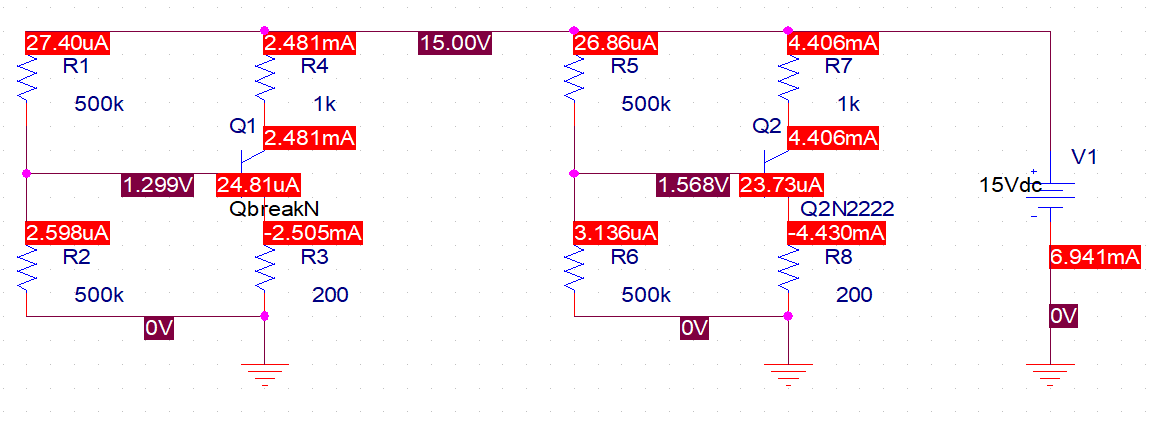
\includegraphics[width=.9\textwidth]{Figures/HW5-5a}
          \caption{Simulation Results for Part (a)}
          \label{fig:1}
        \end{figure}

        From this, we may see that $I_B=23.73[\si{\micro\ampere}]$ and $I_C=4.406[\si{\milli\ampere}]$. Thus, we may obtain:

        $$\beta_{Q2}=\frac{4.406}{.02373}$$
        $$\boxed{\beta_{Q2}=185.67}$$

      \item 

        Once again, we simulate to obtain new values:

        \begin{figure}[H]
          \centering
          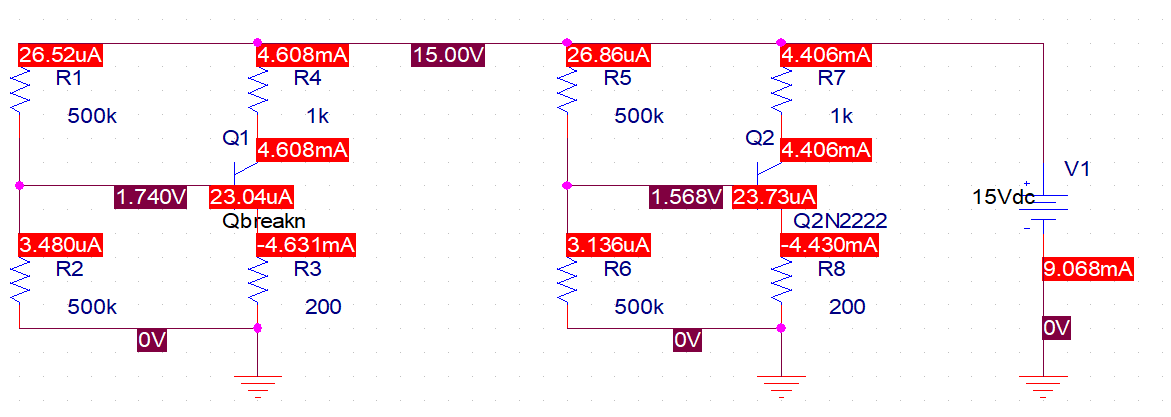
\includegraphics[width=.9\textwidth]{Figures/HW5-5b}
          \caption{Simulation Results for Part (b)}
          \label{fig:2}
        \end{figure}

        Now, we get $I_C=4.608[\si{\milli\ampere}]$ and $I_B=23.04[\si{\micro\ampere}]$, which gives us:

        $$\beta_{QB}=\frac{4.608}{.02304}$$
        $$\boxed{\beta_{QB}=200}$$

        This is the expected value, since we hard coded $\beta$.

      \item 

        We may find the value of BF in the table below:

        \begin{figure}[H]
          \centering
          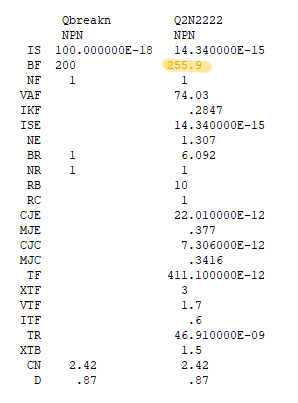
\includegraphics[width=.5\textwidth]{Figures/HW5-5c1}
          \caption{Model Parameters}
          \label{fig:3}
        \end{figure}

        From this, we see that the \underline{expected BF value for the Q2N2222 is 255.9}. Furthermore, we can confirm that BF for the other transistor is 200.

        \begin{figure}[H]
          \centering
          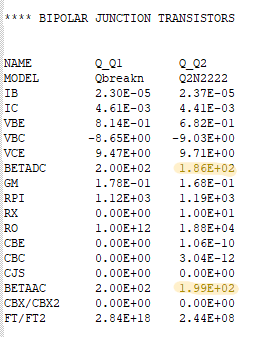
\includegraphics[width=.5\textwidth]{Figures/HW5-5c2}
          \caption{Operating Point Parameters}
          \label{fig:4}
        \end{figure}

        Highlighted in the above figure, we see that BETADC is about 186 and BETAAC is about 199.

      \item 

        The following data sheet was obtained online:

        \begin{figure}[H]
          \centering
          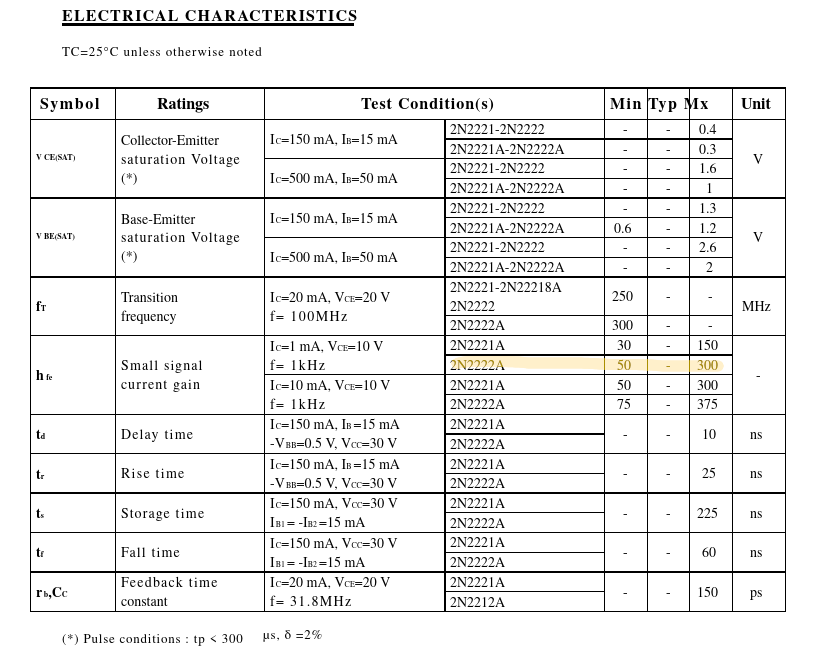
\includegraphics[width=.9\textwidth]{Figures/HW5-5d}
          \caption{Q2N2222 Sample Data Sheet}
          \label{fig:5}
        \end{figure}

        From the highlighted row, we may see that, for $I_C=1[\si{\milli\ampere}]$ and $V_{CE}=10[\si{\volt}]$, the current gain is between 50 and 300. Given that in our simulation $I_C$ is just over 4 times as big, and $V_{CE}$ is about $13.5[\si{\volt}]$, we can estimate that the value will be on the higher end of this range. As observed, $\beta$ was 185.67, which is within the range specified by the data sheet.

    \end{enumerate}

\end{enumerate}

\end{document}

